%03introduction.tex
\renewcommand\thesection{\arabic{section}}
\chapter{Management summary}
\section{Problemstellung}
Je nach Untergrund, Bodeneigenschaften, Gel\"ande sowie Klima gedeihen in der Schweiz unterschiedliche Typen von W\"aldern. Seit einigen Jahrzehnten werden diese Typen von Experten erhoben und kartiert. Es wurden dabei verschiedene typisierte Waldstandorte festgelegt. Aktuell werden Karten, die im Auftrag der Kantone von Experten angefertigt wurden, nur in grossen Intervallen revidiert, wobei sie oft auch nicht fl\"achendeckend vorhanden sind (z.B. in den Kantonen GR, VS, BE).
Einer der Gr\"unde daf\"ur sind u.a. die hohen Kosten, die eine Analyse im Feld mit sich bringt.
Zudem ist die Erfassung und Nachf\"uhrung der Karten gepr\"agt von analogen Vorg\"angen, da die vorhandenen
technischen Ger\"ate und Programme f\"ur den Einsatz im Feld ungeeignet sind.
Daher muss von Hand Niedergeschriebenes im B\"uro oder von staatlichen Institutionen digitalisiert werden, bevor es an den
Arbeitgeber geschickt werden und sp\"ater auf kantonal isolierten Plattformen publiziert werden kann.

\section{Ziel der Arbeit}
Die Erfassung und Publikation von Waldstandorten sollte vereinfacht und beschleunigt werden. Dabei
sollen digitale Technologien eingesetzt werden wie Smartphone, GPS und Internet. Diese neuen
Instrumente sollen entsprechend geschulten Nutzern die Erfassung von Waldstandorten erm\"oglichen sowie \"offentliche und private Informationen in Form von Fl\"achen und Punkten. Auf einer Basis - Karte wird mittels GPS die eigene
Position angezeigt. Dar\"uber werden umliegende, bereits erfasste Waldstandorte, \"offentliche Fl\"achen anderer sowie die eigenen, privaten Fl\"achen dargestellt. Diese Fl\"achen k\"onnen Waldstandorte beschreiben oder aber zus\"atzliche Informationen \"uber den Standort beinhalten, z.B. eine speziell gekennzeichnete Beobachtungsfl\"ache.

\section{Ergebnisse}
Nach einer Evaluation eines Prototyps, erstellt mithilfe eines kommerziellen Produkts,
und der Erstellung von Mockups, wurde ein eigenes Webapp 'Waldmeister Outdoors' realisiert. Durch diese App kann die Arbeit der Experten erleichtert werden. Da die Waldstandort-Karte gleichzeitig im Web synchronisiert
ist, wird dar\"uber hinaus der Informationsaustausch unter allen Beteiligten erleichtert. Die Webapp wurde f\"ur mobile Ger\"ate optimiert und die gew\"unschten Funktionen wurden umgesetzt. Registrierte Benutzer k\"onnen Benutzerfl\"achen in Form von Polygonen direkt auf der angezeigten Map erstellen, mit zus\"atzlichen Informationen versehen und auf einem Server speichern.

\section{Ausblick}
Grosse Teile der Schweiz sind noch unkartiert, und viele Waldstandorte k\"onnten sich unter dem Einfluss der Klimaerw\"armung ver\"andern. Die kontinuierliche Beobachtung solcher Standorte ist Forschungsgegenstand und die Arbeit im Feld ist unerl\"asslich. "Waldmeister - Outdoors" kann im Berufsalltag sowie bei der Kommunikation mit Institutionen den Arbeitsfluss beschleunigen. Weitere Features wie die Verwendung von Plus Codes und offline-F\"ahigkeiten welche bei Verbindungsproblemen zum Einsatz kommen, bzw. Benutzerfl\"achen automatisch synchronisieren, sobald eine Verbindung besteht. Des weiteren bietet es sich an, dass sich User in Gruppen einklinken k\"onnen, um unter sich Benutzerfl\"achen zu teilen und zu besprechen, bevor sie ver\"offentlicht werden. Ebenfalls sollten erstellte Fl\"achen von registrierten Benutzern und deren Gruppen ver\"andert und gel\"oscht werden k\"onnen, nachdem sie erstellt wurden. $\newline$
"Waldmeister - Outdoors" hat das Potential in der Schweiz ein verbreitetes Tool zur Kartierung und Beobachtung von Waldfl\"achen zu werden und stellt eine bereits gefragte Erweiterung der beliebten "Waldmeister" App f\"ur mobile Ger\"ate dar.

\renewcommand\thesection{\thechapter.\arabic{section}}

\chapter{Teil 1 - Technischer Bericht}
\section{Einf\"uhrung}

\subsection{Problemstellung, Vision}
Arbeit im Feld ist, wie bei der Kartierung von Waldstandorten unerl\"asslich ist, wird in allen F\"allen komplementiert von Arbeit, welche ausschliesslich im B\"uro erledigt wird. F\"ur viele Programme existieren ausschliesslich Desktop-L\"osungen, welche auf mobilen Ger\"aten nicht verwendet werden k\"onnen. Wie im Management Summary beschrieben, m\"ussen oft Arbeitsschritte im B\"uro wiederholt werden oder von Hand Niedergeschriebenes am Computer digitalisiert werden. K\"onnten diese Informationen bereits w\"ahrend der Feldarbeit digital festgehalten werde, w\"urde dies die Arbeit sehr verk\"urzen und den Informationsaustausch zwischen verschiedenen Personen und Teams einfacher gestalten.

\subsection{Ziele und Unterziele}
Ziel ist es, eine Webapp zu gestalten, welche es dem User erlaubt bestehende Waldstandorte zu erforschen und nach belieben neue Fl\"achen, welche Waldstandorte beschreiben k\"onnen, zu erfassen. Dies soll auf einem mobilen Ger\"at m\"oglich sein, welches im Feld verwendet wird. Die so erhobenen Daten sollen auf einem zentralen Server gespeichert werden und sofort dem User selbst sowie anderen Benutzern wieder zur Verf\"ugung gestellt werden. Daten, welche so im Feld eingegeben wurden, k\"onnen danach im B\"uro weiterbearbeitet werden. Um dies zu realisieren, wird eine Webapp mit einer Map erstellt, welche je nach User unterschiedliche Informationen auf der Map darstellt. Daten werden vom Client zum Backend \"ubermittelt und in einer Datenbank persistent gemacht, damit sie von einem anderen Ger\"at oder von einem anderen User zu einem sp\"ateren Zeitpunkt zur Verf\"ugung stehen. $\newline$
Das technische Grundger\"ust der App besteht aus einem Client-Server, welcher dem User das Frontend liefert, ein Backend, welches Daten vom User empf\"angt und speichert sowie dem User erm\"oglicht einen Account zu erstellen. Zum Backend geh\"ort ebenfalls eine Datenbank, in welchem s\"amtliche Informationen zu den Waldstandorten und Registrierten Usern gespeichert wird. $\newline$
Ziel ist es, dass die Map auf allen Ger\"aten dargestellt wird und nach erfolgreichem Login Fl\"achen in Form von Polygonen direkt auf der Map erstellt werden k\"onnen. Sie werden vom Backend persistent gemacht und mit dem eingeloggten Benutzer verkn\"upft. Der User kann danach auch auf anderen Ger\"aten auf diese erstellten Fl\"achen zugreifen und sie mit anderen Benutzern teilen.$\newline$

\subsection{Rahmenbedingungen}
Die Software soll auf mobilen Ger\"aten sowie auf Desktop/Laptop Browsern benutzbar sein. Mobile Ger\"ate sind von der Leistung her meist schwach verglichen mit Desktopger\"aten. Server-side rendering kann dieses Problem weniger relevant machen, weil damit die Applikation nicht vollst\"andig vom Client berechnet werden muss. $\newline$
Die Website ist darauf ausgelegt, dass sie im Chrome Browser verwendet wird, da Chrome der verbreitetste Browser auf Android Ger\"aten ist, und auch seine Desktop Version sehr zuverl\"assig funktioniert. Apple Ger\"ate k\"onnen ebenfalls Chrome verwenden. Chrome befindet sich auf den Meisten Ger\"aten auf dem neusten Stand und unterst\"utzt daher die meisten Funktionen. $\newline$
Als Testger\"ate werden ein Apple iPad und iPhone verwendet, ein Android Galaxy S5 und mehrere Macbook Pro und Air Laptops (ca. 2010 - 2016). $\newline$

\subsection{Vorgehen, Aufbau der Arbeit}


\section{Stand der Technik}
\subsection{GIS-Browser}
Ein GIS-Browser, wie er von den verschiedenen Kanton in der Schweiz eingesetzt wird, ist ein read-only Archiv, bestehend aus \"offentlich zug\"anglichen Daten. 
\subsection{ArcGIS online}
Technologien von ESRI (Environmental Systems Research Institute) und insbesondere ArcGIS online (GIS; Geografisches Informationssystem) wurden recherchiert, um einen funktionierenden Prototypen mit offline-caching zu erstellen. Hintergrundkarten (in Form eines Tile-Layers) k\"onnen auf dem Ger\"at zwischengespeichert werden. Die Erstellung von editierbaren Vektorlayern funktioniert auch im offline Betrieb und k\"onnen sp\"ater, sobald wieder eine stabile Internetverbindung besteht, synchronisiert werden. Dieses Verhalten kann bei einer Webapp durch Service-Worker rekreiert werden.$\newline$
Ein GeoJSON (Geo JavaScript Object Notation) file kann ebenfalls auf der online Plattform von ArcGIS hochgeladen werden und danach auf der Map dargestellt werden. Das Layer Styling kann so konfiguriert werden, dass die Farbe eines Polygons dem Typ des jeweiligen Waldstandorts entspricht.
$\newline$
\begin{figure}[H]
    \centering
    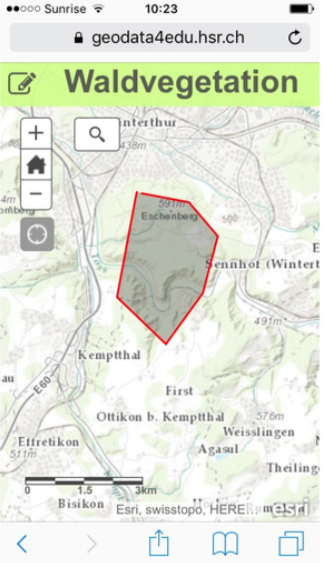
\includegraphics[width=0.5\textwidth]{esriprototyp}
    \caption{Prototyp mit ArcGIS online}
    \label{fig:mesh1}
\end{figure}

\subsection{Defizite}
Ein GIS-Browser wie z.B. vom Kanton Z\"urich bietet keine M\"oglichkeit die eigene Position in Betracht zu ziehen, um damit den Kartenausschnitt zu bestimmen oder genauer noch, den aktuellen Waldstandortstyp per GPS zu bestimmen. Auch ist es nicht m\"oglich, pers\"onliche Notizen oder Fl\"achen wie Beobachtungsfl\"achen zu definieren, damit sie w\"ahrend der Arbeit im Feld verwendet werden k\"onnen. Dies liegt daran, dass sich ein User nicht identifizieren kann, und daher alle Benutzer bei jedem Besuch als anonym behandelt werden.

\section{Bewertung}
\subsection{Kriterien}
\subsection{Schlussfolgerungen}

\section{Umsetzungskonzept}
\subsection{L\"osungsans\"atze}
Webapp (3-Tier Architektur wegen Lernaspekten), Micro-Services, REST-Schnittstelle,  
Native App (Plattformabh\"angig)
\subsubsection{Backend}
Client und Backend sollen Daten per API Abfragen austauschen.
Server als Webservice
\subsubsection{Frontend}
Frontend-Client als Webapp
\subsubsection{Datenbank}
Postgres
SQ-Lite
\subsubsection{JavaScript Libraries}
Vue, Single-Page App
Leaflet, open-source f\"ur Map
Google Maps (Vor-Nachteile)
\subsubsection{Python Pakete}
Django
\subsubsection{Werkzeuge und Tools}
Sublime, Eslint, Flake8, GitHub
\subsubsection{Testing}

\section{Resultate}
\subsection{Zielerreichung}
\subsection{Ausblick und Weiterentwicklung}
\subsection{Pers\"onliche Berichte}
Gdal
\subsection{Danksagungen}
\clearpage
\pagebreak


\chapter{Teil 2 - SW-Projektdokumentation}
\section{Vision}

\section{Anforderungsspezifikationen}
\subsection{Use-Cases}
W\"ahrend der Feldforschung kann es sehr hilfreich sein, auf bereits kategorisierte Waldfl\"achen Zugriff zu haben um sich am Standort zu orientieren. Dieses Material ist oft in einem Kantonalen Portal z.B. https://maps.zh.ch erh\"altlich, es ist jedoch nur selten kompatibel mit mobilen Ger\"aten, interagieren nicht mit dem GPS des Smartphones oder die Websiten sind schwer zu navigieren. "Waldmeister - Outdoors" soll einem gezielten Zweck dienen und nicht mit Kartenmaterial \"uberladen werden. Der Zugriff auf die Vegetationskundlichen Karten sollte vereinfacht und die Navigation beschleunigt werden. $\newline$
Der \"uber GPS ermittelte eigene Standort soll dazu beitragen in dem die eigene Position in der Karte eingetragen werden soll und die Map darauf zentriert wird. Zus\"atzlich soll es m\"oglich sein, dies \"uber einen bestimmten Intervall zu wiederholen, bzw. die eigene Position als Pfad zu speichern. Diese Funktionen sind jedoch stark abh\"angig von der Genauigkeit des GPS, welche innerhalb eines Waldes relativ oft ungenau sein kann, und sollten daher deaktivierbar sein.
\subsection{Must-Haves}
Als must-haves werden Funktionale Anforderungen beschrieben, welche zentrale Funktionen beschreiben, welche ein User mit der Applikation durchf\"uhren m\"ochte. Dazu geh\"oren die Navigation der Map und dem Erstellen und Editieren von Benutzerfl\"achen.
\subsection{Optional}
Als optionale Anforderung wurde das Automatische Anzeige des Waldstandorttyps bezeichnet.
\subsection{Nicht-funktionale Anforderungen}
\subsection{Weitere Funktionen und Anforderungen}
\subsection{Detailspezifikationen}

\section{Analyse}
\subsection{Klassendiagramm}
Das Diagramm \ref{fig:cd1}  schildert die Relation und den Ausbau der wichtigsten Klassen des Systems. Dies zeigt, dass Benutzerfl\"achen nur von registrierten Users erstellt werden k\"onnen und immer einem solchen zugewiesen sind. Wird ein Benutzer aus dem System gel\"oscht, werden alle Fl\"achen welche diesem Account zugeordnet sind , ebenfalls aus dem System gel\"oscht. 

\begin{figure}[h]
\centering
    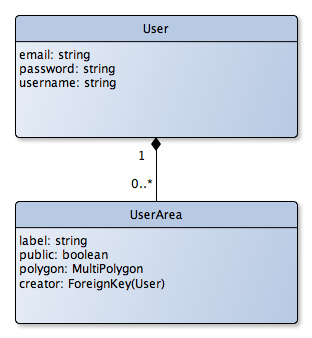
\includegraphics[width=0.5\textwidth]{ClassDiagram2}
    \caption{Klassendiagramm}
    \label{fig:cd1}
\end{figure}

\subsection{Domain Modell}

\section{Technologien}
\subsection{Django}
Als Server zur Verwaltung der User und der Daten, welche die User generieren und ben\"otigen, kommt Django zum Einsatz. Es ist ein Open-Source Webframework, welches das Python Gegenst\"uck zu Ruby-On-Rails darstellt. Im Kern folgt es dem Model-View-Controller Prinzip, obwohl es eine eigene Namensgebung Verwendet. \cite{django1} In diesem Projekt verwendet Django eine PostgreSQL Datenbank um Daten persistent zu machen. Django wird ebenfalls dazu verwendet um User einen Account zu geben, damit nur sie selbst Zugriff auf Ihre privaten Benutzerfl\"achen haben, oder um \"offentlich erstellte Benutzerfl\"achen mit anderen zu teilen. $\newline$

\subsubsection{Django Rest Framework}
Eine SPA kommuniziert haupts\"achlich \"uber API Schnittstellen mit dem Server. Hier kommt auf dem Server das Django Rest-Framework (DRF) zum Einsatz. $\newline$
Es bietet ein sehr flexibles System zur Erstellung von RESTful Web-APIs. Das DRF bietet die M\"oglichkeit CRUD Operationen auf eine Ressource auszuf\"uhren. "Waldmeister - Outdoors" verwendet die REST Api beispielsweise um usergenerierte Fl\"achen, Pfade oder Punkte in der Datenbank zu speichern oder diese zur Darstellung in der Map aus der Datenbank zu laden. $\newline$
Ebenfalls werden Benutzer welche sich registrieren, mit Username, Password und ggf. Emailadresse in der Datenbank eingetragen. $\newline$

\subsection{PostgreSQL}
Postgres ist das Datenbank Management System, welches mit Django zusammen die Daten persistent macht, welche die User per API in der PWA generieren. Hierzu wird das Django Packet psycopg2 verwendet. Django kann durch Models ein Datenbankschema beschreiben, welches von PostgreSQL generiert und in einer lokalen PostgreSQL Instanz gespeichert wird. \cite{pg1} \cite{django2}

\subsubsection{PostGIS}
Um Geoinformationsdaten wie z.B. Polygone und Pfade korrekt zu speichern wird auf der Datenbank das Plugin PostGIS installiert. Dadurch kann Django die ben\"otigten Datenbankmodelle erstellen und per REST Schnittstelle speichern. Anhand des Django Models werden Geodaten in einem gew\"ahlten Format gespeichert. Standardm\"assig wird von Django die Spatial Reference Identifier (SRID) Nummer 4326 (World Geodetic System, WGS84) verwendet. Dieses System benutzt Zahlen von -180, -90 bis 180, 90 um Positionen auf der Erde (in Latitude und Longitude) zu beschreiben. $\newline$
Postgis wird ebenfalls dazu verwendet, dass die Daten, welche per REST-Schnittstelle an den Client geschickt werden, in richtigem Format (Multipolygone in GeoJSON) \"ubermittelt werden.

\subsection{VueJS}
Vue.JS ist ein JavaScript Framework, welches sich zum Erstellen von Single-Page-Webapplikationen in Form einer PWA eignet. Es wurde im Jahr 2013 erstmals ver\"offentlicht und wurde am 19. Dezember 2017 auf die aktuellste Version 2.5.13 gepatcht. Vue.JS folgt einer Variation des Model-View-Controller-Entwurfmusters, dem Model - View - ViewModel Muster. Wie auch das MVC folgt MVVM dient es der Trennung von Darstellung und der Logik der Benutzerschnittstelle. Dies erlaubt dem nutzenden Entwickler, die Struktur der Anwendung nach eigenen Anspr\"uchen zu richten. $\newline$
Entwickler beschreiben es daher als "less opinionated" im Vergleich zu anderen popul\"aren JavaScript Webframeworks wie Anglar.JS oder React. Vue.JS kann von Entwicklern eingesetzt werden welche HTML und JavaScript beherrschen und erfordert keine weiteren Webtechnologien. Vue.JS setzt eine Website aus Instanzen und Komponenten, bzw Single File Components zusammen. Single File Components sind bei VueJS, welche Architekturprobleme von mittel bis grossen Webapps, welche vollst\"andig von JavaScript getrieben werden, zu verbessern versucht. $\newline$
Folgende Probleme tauchen dabei auf:
$\newline$
\begin{enumerate}
\item Global definitions $\newline$
Global definitions force unique names for every component
\item String templates $\newline$
String templates lack syntax highlighting and require ugly slashes for multiline HTML
\item No CSS support $\newline$
No CSS (Cascading Style Sheets) support means that while HTML and JavaScript are modularized into components, CSS is conspicuously left out
\item No build step $\newline$
No build step restricts us to HTML and ES5 JavaScript, rather than preprocessors like Pug (formerly Jade) and Babel
\end{enumerate}
$\newline$
VueJS besagt, dass all diese Probleme von Single File Components (mit .vue extension) dank Werkzeugen wie Webpack und Browserify gel\"ost werden. Eine solche Komponente besteht auf HTML Template, JavaScript und CSS in einer eigenen, abgekapselten Datei. 
$\newline$
Durch das erzielt VueJS $\newline$

\begin{enumerate}
\item Complete syntax highlighting
\item CommonJS modules
\item und Component-scoped CSS
\end{enumerate}

Wem diese Idee Abkapselung nicht gef\"allt, der kann weiterhin ein CSS auslagern und in eine Komponente (innerhalb des HTML Templates) importieren: $\newline$
\begin{lstlisting}
<!-- my-component.vue -->
<template>
  <div>This will be pre-compiled</div>
</template>
<script src="./my-component.js"></script>
<style src="./my-component.css"></style>
\end{lstlisting}
$\newline$

\subsubsection{Separation of Concern}
Was ist gemeint mit Separation of Concern (SoC) und bricht der Aufbau von Single-File-Components nicht dieses Pattern? Eine bekannte Vorgehensweise bei Softwareengineering ist es, ein Computerprogramm in logische Abschnitte einzuteilen und zu separieren. Diese Teile sollten sich um einen Zweck oder Belang (Concern) k\"ummern. Dies heisst jedoch nicht, dass die verschiedenen Dateitypen unbedingt in separate Dateien aufgeteilt werden. In der modernen User Interface Entwicklung und den Entwicklern von VueJS ist es oft einfacher gefallen, verschiedene Komponenten, welche lose gekoppelt sind, zu komponieren, statt sie auf drei riesigen Layern (HTML, JS und CSS) getrennt zu halten, sie aber in den Komponenten zu verflechten. \cite{VueSFC} $\newline$
Auf diesem Weg sind Komponenten (Template, die Logik und das Styling) zusammenh\"angender und auch einfacher zu warten, obwohl dies nicht den Prinzipien von SoC folgt. Traditionelles SoC unterteilt dies in die Gruppen der Zwecke Organisation (HTML), Pr\"asentation (CSS) und Interaktion bzw. Verhalten (JavaScript).

\subsubsection{Vue-Router}
Der Vue-Router ist das Herzst\"uck einer Single-Page-Applikation (SPA). Der offizielle Vue-Router ist ein Client-seitiger Router, welcher mithilfe der HTML5 History API voll funktionsf\"ahiges Client-side routing macht. $\newline$ In der HTML Definition der Hauptkomponente kann <router-view> als Platzhalter verwendet werden, um die Komponenten anzuzeigen, welche abh\"angig von der momentanen Route an dieser Stelle angezeigt werden sollen. Ein Wechsel zwischen diesen Routen bewirkt kein Page-Reload, da dies von Vue.JS lediglich innerhalb derselben Page \"Anderungen bewirkt und keine tats\"achlichen URL Aufrufe ausf\"uhrt. $\newline$
Der Vue Router wird innerhalb einer Hauptseite angezeigt welche die Basis der Webseite darstellt. Methoden von Komponenten k\"onnen bewirken, dass sich der Inhalt ver\"andert, welcher an der Stelle des Router-Views angezeigt wird. Menupunkte im Header (z.B Register, Login, About, Map), bewirken mit .push() dass der Vue-Router mithilfe des index.js files die korrekten Komponenten an dieser Stelle anzeigt. Dies kann auch direkt \"uber eine URL Eingabe /register oder /login erfolgen, ohne dass der Aufruf \"uber eine interne Komponente ausgef\"uhrt werden muss. Die Datei index.js beinhaltet daher alle m\"oglichen Pfade, welche von der Webapp aufgel\"ost werden und bestimmt die angezeigten Komponenten, welche mit dieser Route verkn\"upft sind. $\newline$
Alternativ k\"onnten die \"ahnlichen L\"osungen von Page.js oder Director als Third-Party Produkte an dieser Stelle integriert  werden, es ist jedoch zu empfehlen, die offizielle Vue-Router Library zu verwenden.

\subsubsection{VueX}
VueX ist eine offizielle Erweiterung von Vue.JS und fungiert als Statusmanager. VueX arbeitet mit einem Store, welcher die Zust\"ande aller Komponenten in einer Vue Applikation \"uber Regeln definiert. VueX besteht aus Actions, Mutations und States. Aktionen k\"onnen in dieser Reihenfolge eine Auswirkung auf die Vue Komponenten haben. $\newline$
VueX hat Vorteile bei mittel bis grossen Projekten, welche auf dem Single-Page-Application Prinzip basieren. VueX bietet auch die M\"oglichkeit, einen zentralen Store in kleinere Module aufzuteilen, jedes mit ihren eigenen State, Mutations, Actions Werten. $\newline$
Da Komponenten in Vue abgekapselt sind, k\"onnen sie standardm\"assig nicht auf Daten zugreifen ,welche in anderen Komponenten definiert werden. Solche Daten m\"ussen per Store verf\"ugbar gemacht werden, damit sie \"uber mehrere Instanzen geteilt werden k\"onnen. $\newline$

\begin{lstlisting}
const sourceOfTruth = {}

const vmA = new Vue({
  data: sourceOfTruth
})

const vmB = new Vue({
  data: sourceOfTruth
})
\end{lstlisting}
$\newline$

Wird nun sourceOfTruth ver\"andert, wird sie in allen Komponenten, in welcher sie verwendet wird, automatisch auf den neuen Stand gebracht. Dies kann in gr\"osseren Applikationen schnell un\"ubersichtlich werden, da jede Komponente diese sourceOfTruth ver\"andern kann, ohne eine nachvollziehbare Spur zu hinterlassen. Es wird daher empfohlen, das Store Pattern von VueX zu implementieren, welche Ver\"anderungen am Store nur \"uber Mutationen zul\"asst. Somit wird es klarer, zu welcher Zeit welche Mutationen aufgerufen werden k\"onnen und wie sie durchgef\"uhrt wurden:$\newline$

\begin{lstlisting}
var store = {
  debug: true,
  state: {
    message: 'Hello!'
  },
  setMessageAction (newValue) {
    if (this.debug) console.log('setMessageAction triggered with', newValue)
    this.state.message = newValue
  },
  clearMessageAction () {
    if (this.debug) console.log('clearMessageAction triggered')
    this.state.message = ''
  }
}
\end{lstlisting}
$\newline$

\begin{figure}[H]
    \centering
    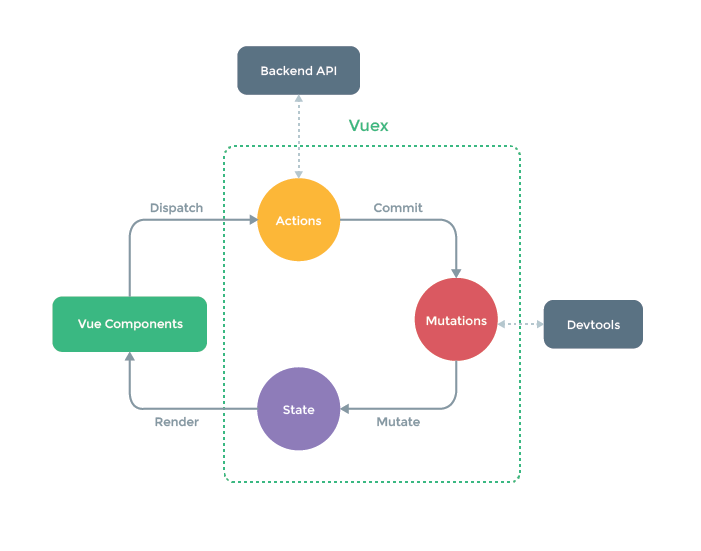
\includegraphics[width=1.25\textwidth]{vuex}
    \caption{Vuex Action-Mutations-State Diagram}
    \label{fig:mesh1}
\end{figure}

Komponenten k\"onnen auch private Zust\"ande haben, dies wird mit "privateState" erreicht. In diesem Fall muss der sharedState ebenfalls definiert werden.

\begin{figure}[H]
    \centering
    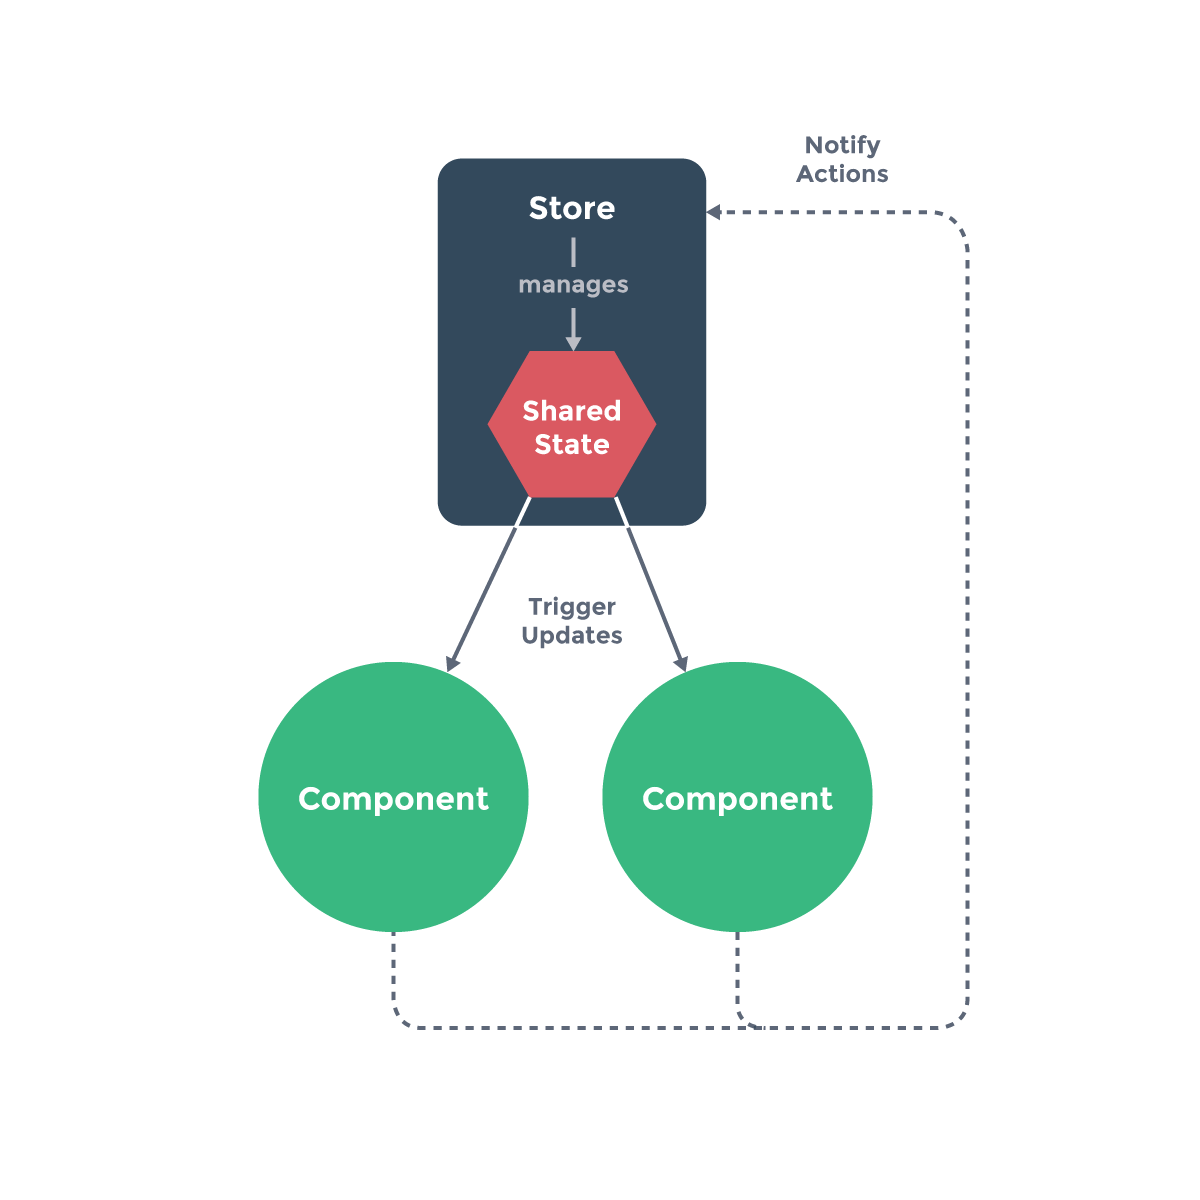
\includegraphics[width=1.25\textwidth]{sharedstate}
    \caption{Vuex private}
    \label{fig:mesh2}
\end{figure}

Dies bewirkt, dass eine Komponente nicht direkt einen Wert oder Zustand im Store ver\"andern kann, sondern dies einen Event aufruft. Dieser informiert den Store welchen State es \"uber eine Mutation zu ver\"andern gilt.

\subsubsection{Docker}


\section{Design}
\subsection{Architektur}
\subsection{Objektkatalog}
Waldstandort: Eine Fl\"ache auf der Erdoberfl\"ache, welche einen Walddarstellt $\newline$
Waldstandortstyp: Einer von vielen Typen, welcher einen Waldstandort einen bestimmten Typ zuordnet. Meist wird hier der K\"urzel aus den Definitionen von ek72 verwendet, z.B. K\"urzel "7e". Der volle Name des Waldstandortstyps "7e" ist "Waldmeister-Buchenwald mit Hornstrauch"
\subsection{Package Struktur}
Der Source-Code von "Waldmeister-Outdoors" ist auf GitHub unter "https://github.com/dschmide/Waldmeister-Outdoors" erh\"atlich. Die Paket-Struktur des Projekts ist in die Teile "backen", "client", "Dokumentation" und "secured-local-nginx" aufgeteilt.
$\newline$
screenshots

\subsection{Sequenz-Diagramm}


\subsection{UI Design}
\subsubsection{Mockups}
Die Mockups wurden vor der Implementation erstellt, um Screendesign und Layout klarer zu definieren, bevor es um die technische Implementation von "Waldmeister - Outdoors" ging. In den Abbildungen 1 bis 9 kann man den Arbeitsschritt Einloggen und Erstellen einer neuen Fl\"ache und eines Points of Interests (POI) sehen. Zus\"atzlich sieht der User seine eigene Location auf der Map eingetragen und hat \"uber das Menu "My Places" Zugriff auf eine Liste seiner erstellten Fl\"achen. Ein Kontextmenu gibt bei der Anzeige eines ausgew\"ahlten Objekts zus\"atzliche Informationen.

\pagebreak

\begin{figure}[H]
\centering
    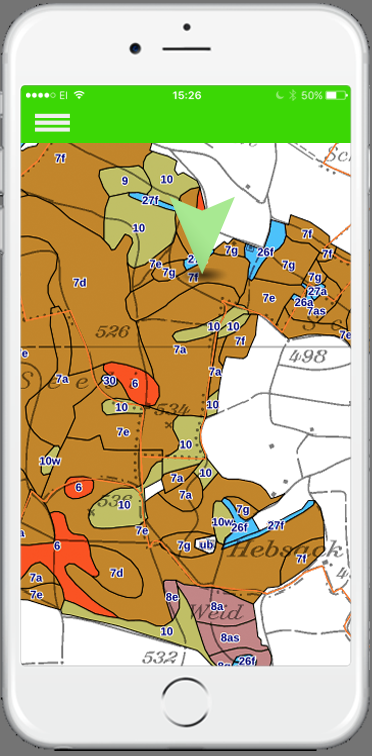
\includegraphics[width=0.7\textwidth]{mockup1-1}
    \caption{Mockup Screen 1}
    \label{fig:mesh1}
\end{figure}

\begin{figure}[H]
\centering
    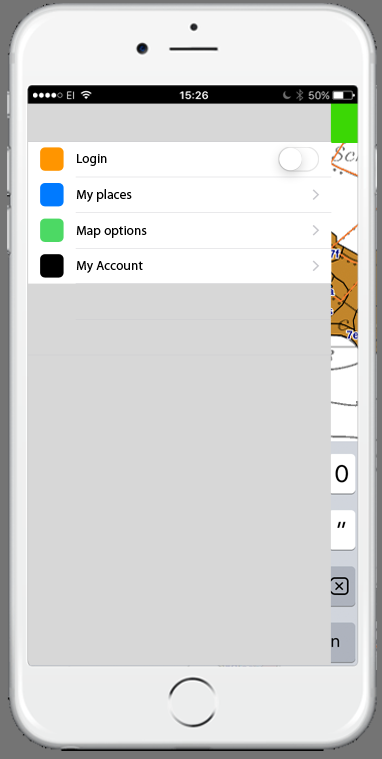
\includegraphics[width=0.7\textwidth]{mockup1-2}
    \caption{Mockup Screen 2}
    \label{fig:mesh2}
\end{figure}

\begin{figure}[H]
\centering
    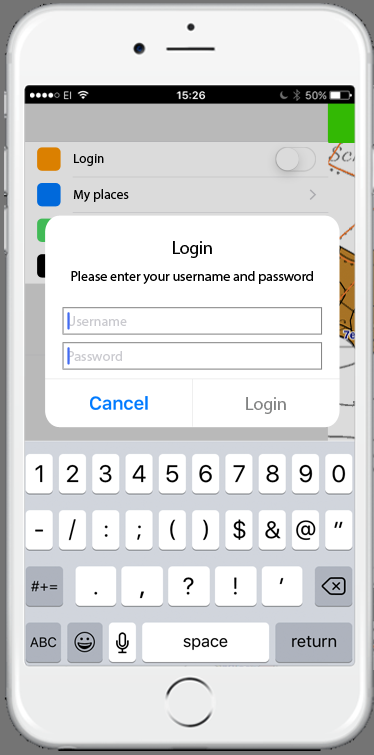
\includegraphics[width=0.7\textwidth]{mockup1-3}
    \caption{Mockup Screen 3}
    \label{fig:mesh3}
\end{figure}

\begin{figure}[H]
\centering
    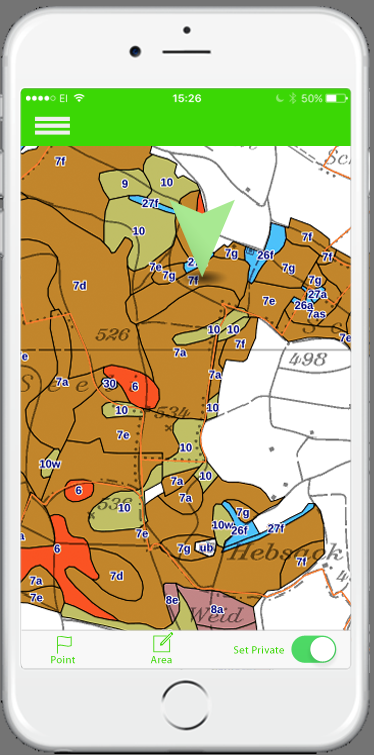
\includegraphics[width=0.7\textwidth]{mockup1-4}
    \caption{Mockup Screen 4}
    \label{fig:mesh4}
\end{figure}

\begin{figure}[H]
\centering
    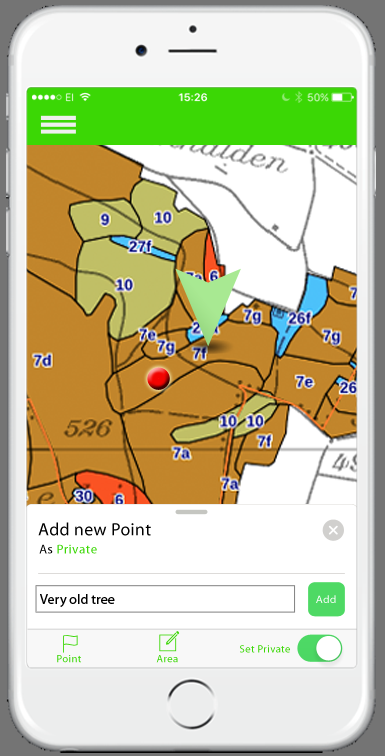
\includegraphics[width=0.7\textwidth]{mockup1-5}
    \caption{Mockup Screen 5}
    \label{fig:mesh5}
\end{figure}

\begin{figure}[H]
\centering
    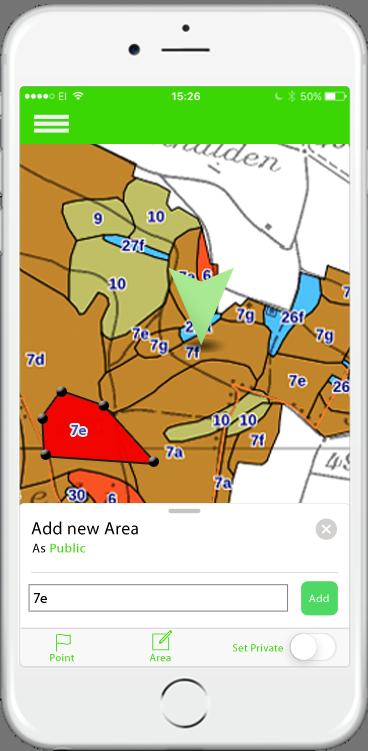
\includegraphics[width=0.7\textwidth]{mockup1-6}
    \caption{Mockup Screen 6}
    \label{fig:mesh6}
\end{figure}

\begin{figure}[H]
\centering
    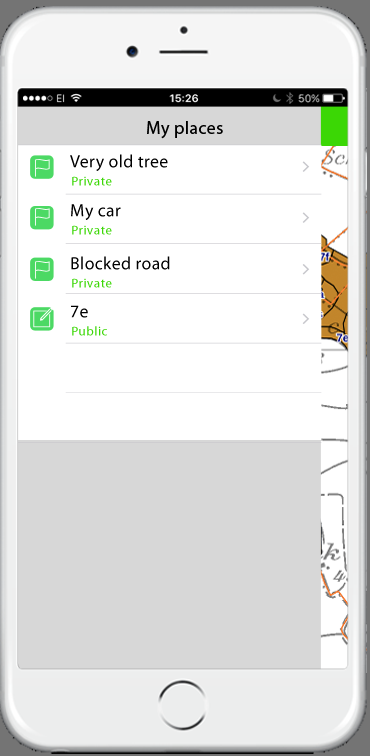
\includegraphics[width=0.7\textwidth]{mockup1-7}
    \caption{Mockup Screen 7}
    \label{fig:mesh7}
\end{figure}

\begin{figure}[H]
\centering
    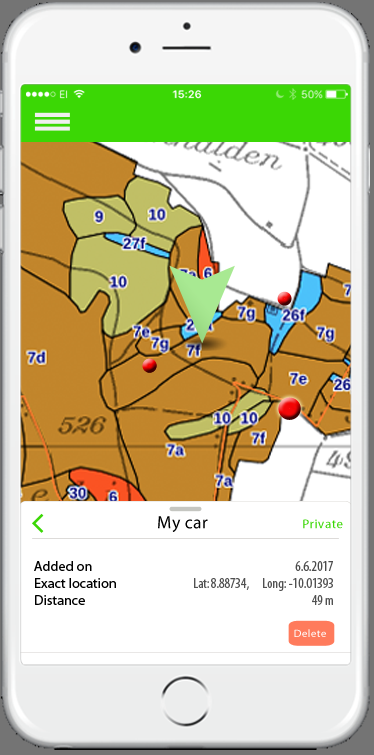
\includegraphics[width=0.7\textwidth]{mockup1-8}
    \caption{Mockup Screen 8}
    \label{fig:mesh8}
\end{figure}

\begin{figure}[H]
\centering
    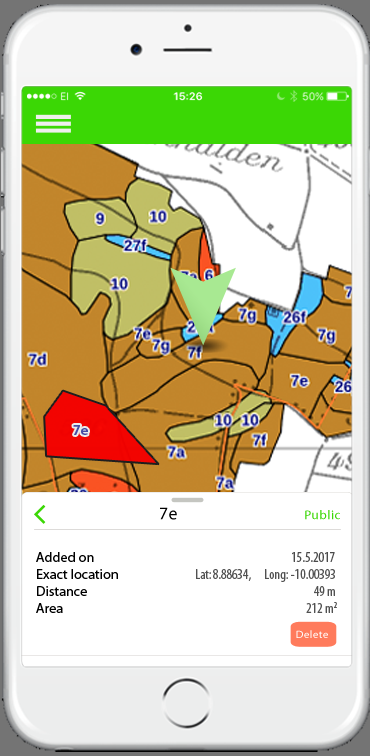
\includegraphics[width=0.7\textwidth]{mockup1-9}
    \caption{Mockup Screen 9}
    \label{fig:mesh9}
\end{figure}

\section{Implementation und Test}
\subsection{Implementation}
\subsubsection{Technische Implementation}
\subsubsection{API und Datenquellen}

\subsubsection{Vue Komponenten}
Die Applikation "Waldmeister - Outdoors" setzt sich aus den Komponenten Register, Login, About, der WaldmeisterMap und einem Page Header zusammen. Dar\"uber hinaus bildet die Komponente "App.vue" die Basis, um den Page Header und Router-View Komponenten zu laden. $\newline$
\subsubsection{Registrierung und Login}

Registrierung und Login wurden als separate Single-File-Komponenten aufgebaut, damit sie vom Vue-Router dargestellt werden k\"onnen. Sie beinhalten die Felder Username, Passwort und bei der Registrierung auch ein Email Feld, welches optional ist. Bei der erfolgreichen Registrierung wird von Djoser ein Benutzer angelegt und sein Passwort im verschl\"usselten Zustand hinterlegt. Loggt sich der Benutzer mit den korrekten Daten ein, erh\"alt er vom Server ein JWT (JSON Web Token), welches von Djoser basierend auf dem hinterlegten Accounts erstellt wird. Der Vue-Client Server hinterlegt dies in einem Store, damit es in verschiedenen Komponenten verwendet werden kann. Um sich dem Server gegen\"uber zu authentifizieren wird es bei einem Request mitgeschickt. Loggt er sich aus, wird dieses aus dem Store gel\"oscht. Der User kann sich erneut oder unter einem anderen Benutzernamen und Passwort einloggen. $\newline$
Bei nicht erfolgreichen Versuchen, einen Account zu erstellen oder sich einzuloggen, werden dem User diverse Fehlermeldungen angezeigt, welche Auskunft \"uber fehlerhafte Passworteingabe oder Benutzerdaten bei der Erstellung des Accounts geben. $\newline$
Nach einem erfolgreichen Login wird der User per Vue-Router auf die Komponente WaldmeisterMap weitergeleitet und alle Benutzerfl\"achen werden vom Server angefordert, auf die er Zugriff hat. Der Server liefert per REST Interface alle \"offentlichen Benutzerfl\"achen, sowie die privaten Benutzerfl\"achen, welche diesem User zugeordnet sind. \cite{djoserpack} $\newline$

\subsubsection{Map Komponente}
Die Komponente WaldmeisterMap ist die Komponente, auf welcher die Leaflet Map und darauf die Layer Vegetationskarte (als geoJSON) und der Layer f\"ur die Benutzerfl\"achen (als Polygone) dargestellt werden. Das leaflet Map Objekt beinhaltet auch die Kontrollbuttons, welche mit der Map assoziiert sind. Durch die Buttons 'Veg' und 'Areas' in der oberen linken Ecke der Map k\"onnen die GeoJSON bzw die Benutzerfl\"achen ein - und ausgeschaltet werden. Dadurch werden die Layer, auf welchen sich die Polygone befinden gecleart und alle erstellten Labels von der Map gel\"oscht. Bet\"atigt der User den Button noch einmal, werden sie erneut erstellt. Sie sind standardm\"assig eingeschaltet und werden daher auch erstellt, wenn das Map Objekt auf die Page gemountet wird (beim Laden der WaldmeisterMap Komponente). Damit Label und Polygone der verschiedenen Layer separat ein und ausgeschaltet werden k\"onnen, werden sie zuerst in Gruppen unterteilt, bevor diese Gruppen auf die Map hinzugef\"ugt werden.$\newline$
Oberhalb dieser zwei Buttons befindet sich der "Add" Button, welcher es dem User erm\"oglicht, eine neue Benutzerfl\"ache auf der Map einzutragen. Er kann, w\"ahrend er im Zeichnungsmodus ist, per click event dem Polygon einen neuen Eckpunkt anh\"angen. Klickt der User w\"ahrend des Zeichnungsmodus auf den ersten erstellten Eckpunkt, schliesst sich das Polygon und der User wird per Dialogbox aufgefordert, dem erstellten Objekt die ben\"otigten Attribute zuzuweisen (label, public). Dr\"uckt er in diesem Dialog auf "Save" wird die Fl\"ache an den Server geschickt und in der Datenbank gespeichert. $\newline$

\subsubsection{About}
Die Komponente About enth\"alt wichtige Informationen zu den dargestellten Daten und beinhaltet die Links zu den nativen iOS und Android Apps, unter welchen das Nachschlagewerk "Waldmeister" erh\"altlich ist. Unterhalb des dargestellten Logos befinden sich ausserdem Informationen zum Projekt und den Rahmenbedingungen, unter welchen es erstellt wurde. $\newline$
Hier wird auch dem Kanton Z\"urich gedankt f\"ur die Nutzungsrechte der Daten "Vegetationskundliche Kartierung der Waldfl\"achen im Kanton Z\"urich".

\begin{figure}[H]
\centering
    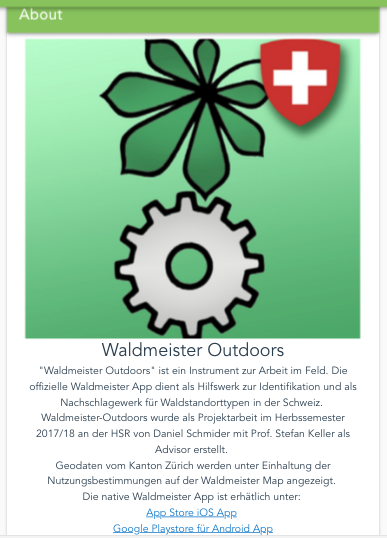
\includegraphics[width=0.5\textwidth]{aboutscreen}
    \caption{About in der Waldmeister-Outoors Webapp}
    \label{fig:aboutscreen}
\end{figure}

\subsubsection{Frontend}
Das User Interface wurde gr\"osstenteils mit Vuetify realisiert, welches die \"aussere Erscheinung der Komponenten Header, Registrierung, Login, About, etc... bestimmt. Es wurde auf das Farbschema der existierenden Waldmeister App angepasst und eignet sich um eine Webapp responsive zu gestalten, damit sie auf mobilen Ger\"aten ebenfalls korrekt dargestellt wird. $\newline$
Weitere Teile, vor allem Elemente welche sich auf der Leaflet Map befinden, wurden mit CSS Styling aufgewertet. Der GeoJSON Layer, welcher die Fl\"achen der Waldstandorte anzeigt, wird durch CSS dazu verwendet jedes Polygon auf diesem Layer aufgrund von einem Property des Polygons einzuf\"arben. Dieses Property ist die EK72 Kennzahl, bzw. K\"urzel. Jedem dieser K\"urzel kann eine bestimmte Farbe zugewiesen werden, welche als hexadezimale, 6-tellige Zahl im Code repr\"asentiert wird. Jedes Polygon erh\"alt dar\"uber hinaus auch ein Label, welches dieses K\"urzel ebenfalls darstellt. Diese Property Label haben eine weisse Schrift, sind nicht transparent und haben einen 2 Pixel weiten Schatten, damit sie sich von der Hintergrundfarbe abheben.$\newline$

\begin{figure}[h]
\centering
    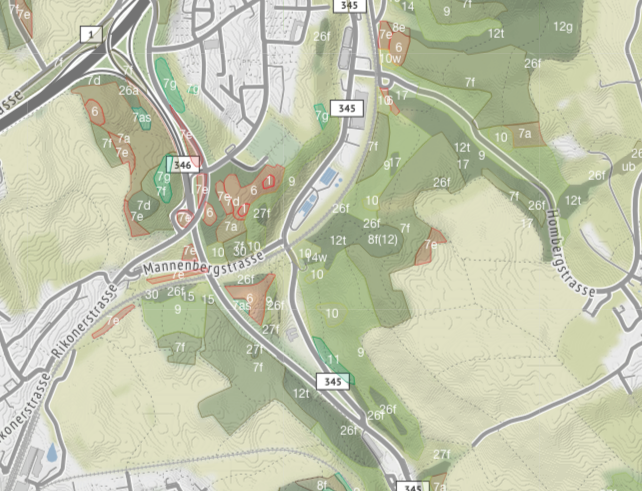
\includegraphics[width=1\textwidth]{propertylabel}
    \caption{Einf\"arbung von GeoJSON Fl\"achen und Darstellung von PropertyLabels}
    \label{fig:propertylabel}
\end{figure}

$\newline$
Benutzerfl\"achen werden blau dargestellt und haben ein gef\"arbtes Label, damit sie sich von den Fl\"achen des geoJSON Layers unterscheiden. Private Fl\"achen haben ein gelbes Label, \"offentliche sind gr\"un. Dar\"uber hinaus haben sie eine breitere Outline als Fl\"achen des GeoJSON Layers.

\begin{figure}[H]
\centering
    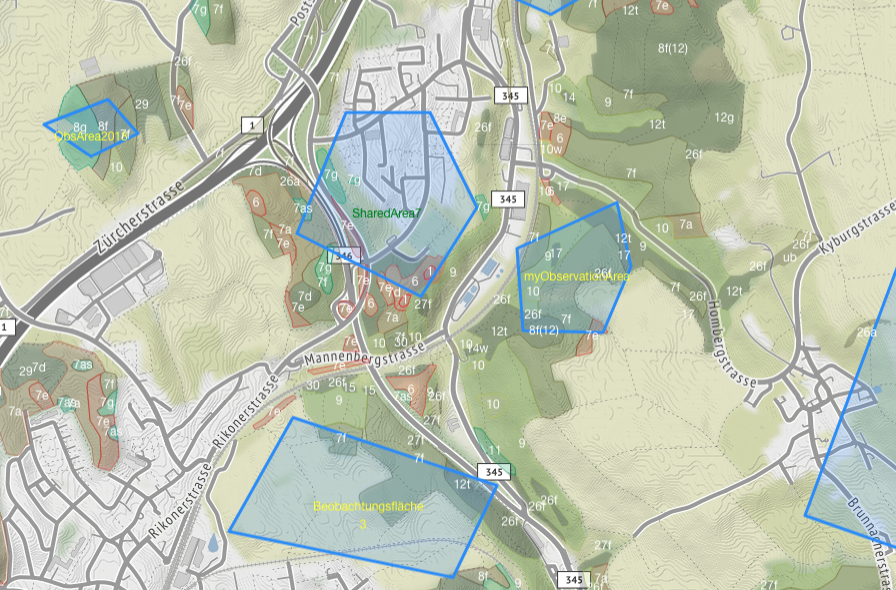
\includegraphics[width=1\textwidth]{userareas}
    \caption{Benutzerfl\"achen mit Labels}
    \label{fig:userareslabels}
\end{figure}

Die Geolocation wird als blauer "Circle" dargestellt. Die Gr\"osse des Kreises repr\"asentiert die Genauigkeit der Berechnung der Geolocation in Metern. $\newline$

\begin{figure}[H]
\centering
    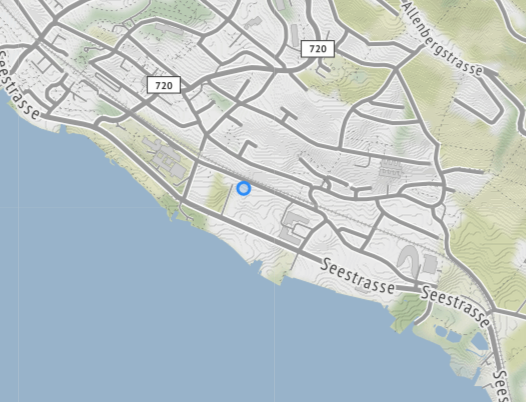
\includegraphics[width=1\textwidth]{geolocation}
    \caption{Geolocation mit Circle}
    \label{fig:geoloc1}
\end{figure}

Die Buttons welche den Zeichungsmodus starten oder beenden oder Ebenen ein- und ausblenden sind in der oberen linken Ecke, unterhalb der Zoombuttons vertikal aufgereiht. Der Zeichnungsbutton ist mit "Add" beschriftet und wechselt auf "Edit" solange der Zeichnugsbutton aktiviert ist. Die Buttons zum Ein- und Ausblenden von Ebenen sind mit "Veg" und "Areas" beschriftet, haben aber l\"angere Tooltips, welche die Funktion genauer beschreiben. $\newline$

Die "Save" Dialogbox wird nur angezeigt, wenn eine gezeichnete Fl\"ache durch einen Klick auf den ersten gezeichneten Eckpunkt geschlossen wird. Durch den "Save" Button innerhalb der Dialogbox werden die Werte f\"ur Label und Public \"ubernommen und das gezeichnete Polygon wird per REST Schnittstelle an den Server geschickt, damit es in der Datenbank gespeichert wird.

\subsubsection{Axios Requests}
Diese Anfragen werden vom Client \"uber eine Axios API abgesetzt. Nach der Initialisierung des Axios Services wird eine Base Url bestimmt, welche auf das Backend im Django Server zielt. Mit jedem Request, welches \"uber diesen Service ausgef\"uhrt wird, wird auch das im Store hinterlegte JWT Token mitgeschickt, sofern es existiert. Falls nicht, wird der User als nicht autorisiert identifiziert.
Neben der Authentication Service, welcher die Methoden Register und Login ausl\"osen kann, besteht der AreaService, welcher per getAreas und postAreas Benutzerfl\"achen vom Server anfordern oder an den Server schicken kann, damit sie in der Datenbank erstellt werden. Die Erstellung von neuen Fl\"achen ist jedoch nur m\"oglich, wenn der User sich eingeloggt hat.$\newline$
Abh\"angig vom Request f\"ugt Axios Service eine URL-Endung an die Basisurl an, damit Django per Routingsystem erfassen kann um welche Art Request es sich handelt. Post Requests innerhalb des AuthenticationServices kommunizieren mit den Djoser definierten URL-Endungen /auth/users/create (um beispielsweise einen neuen Benutzer zu registieren). Diesem Post Request werden die credentials mitgeschickt, welche vom User im Client eingegeben wurden. Dieses credentials-Objekt besteht aus username, password und email. Sie werden als JSON Objekt an den Django Server geschickt.$\newline$
Neben dem AuthenticationService regelt der AreaService per get und post requests \"uber die URL-Endungen '/api/areas/' Requests bez\"uglich Benutzerfl\"achen.
Axios kommuniziert mit dem Server \"uber eine REST-Schnittstelle. Benutzerfl\"achen werden per Get-Request an den Client \"ubertragen, neu erfasste Benutzerfl\"achen werden \"uber einen Post-Request als JSON Objekte an den Server \"ubertragen. Django deserialisiert diese JSON Objekte und speichert sie anschliessend in der PostgreSQL Datenbank. $\newline$

\subsubsection{Database Models}
Die Benutzerfl\"achen werden von Django durch ein Django-Dabatase-Model beschrieben und haben die Attribute "label, public, polygon und creator".  Label ist ein Feld welches aus Charakteren und Ziffern besteht. Die Maximall\"ange ist auf 50 Zeichen gesetzt, kann aber beliebig erh\"oht werden. $\newline$
Das Feld 'public' ist ein Boolean Wert, welcher bestimmt, ob eine Fl\"ache \"offentlich oder privat gehandhabt wird. $\newline$
'polygon' beinhaltet die Geometrie, die Art der Fl\"ache und das Format, in welcher sie in der Datenbank gespeichert wird. Die Geometrie ist Teil des polygon field und beinhaltet ein Array welches Punkte in Longitude / Latitude Paaren enth\"alt, die die Ecken des Polygons beschreiben. Dies k\"onnen beliebig viele sein und im Falle eines Multipolygons kann dieses Feld auch mehrere Arrays beinhalten, welche wiederum ein einzelnes Polygon beschreiben. \"Uberschneiden sich mehrere Polygone entstehen "Inseln", welche nicht zu der Fl\"ache des Multipolygons geh\"oren.$\newline$
Also Koordinatensystem wird das System WGS84 mit der SRID 4326 verwendet. \site{srid}

\subsubsection{Database, PostgreSQL}
Nachdem die Datenbank Modelle von Django definiert wurden, m\"ussen sie \"uber einen migrate Befehl in die PostgreSQL Datenbank \"ubertragen werden, damit sie erstellt werden. F\"ur die Kommunikation zwischen Django und PostgreSQL wird das Python Package Psycopg2 verwendet. Dieses Package ist der verbreitetste PostgreSQL Datenbank Adaptor f\"ur die Python Programmiersprache. $\newline$
Als Datenbank wird PostgreSQL 10 verwendet. Die Datenbank Verbindungsdetails sind in der Python settings.py Datei eingetragen. Waldmeister-Outdoors wird versuchen, auf eine lokale Datenbank mit dem Namen 'dschwaldmeister' zuzugreifen. Username ist postgres und der Port ist auf 5435 gesetzt, um Komplikationen mit anderen lokalen PostgreSQL Installationen zu vermeiden. Die "Engine" wurde ebenfalls auf 'django.contrib.gis.db.backends.postgis' ge\"andert, da postgis auf der Datenbank verwendet wird und als Extension installiert werden muss. Mit psql \"uber die Konsole oder PGAdmin4 k\"onnen auf die lokale PostgreSQL Datenbank zugegriffen, Daten manuell gel\"oscht oder eingetragen werden.

\subsubsection{Kartenmaterial}
\subsubsection{etc.}

\section{Automatische Testverfahren}
Testgetriebene Entwicklung (TDD) ist eine Methode zur Softwareentwicklung, welche oft bei der agilen Entwicklung von Computerprogrammen eingesetzt wird. Bei TDD erstellt der Programmierer Software-Tests, um das korrekte Verhalten von Softwarekomponenten zu planen und zu \"uberpr\"ufen. Unit Tests (auch als Unittest oder als Komponententest bezeichnet), werden verwendet um die funktionalen Einzelteile eines Softwareprojekts zu pr\"ufen. 

\subsection{Django}
Test f\"ur das Django wurden mit dem standard Django module "unittest" erstellt. Es wurden Tests zu Login, Registrierung und Erstellung von Benutzerfl\"achen erstellt. Es werden unvollst\"andige, fehlerhafte und nicht authorisierte Requests (zum Beispiel ohne sich einzuloggen) getestet. HTTP-Statuscode geben Auskunft \"uber die korrekte Ausf\"uhrung oder fehlerhaftes Verhalten des Servers. Sie werden verglichen mit zu erwartenden Codes und bestimmen auf diese Weise ob der Test bestanden oder gescheitert ist. $\newline$
$\newline$
Es wird getestet ob Email und Passwort vorhanden ist und ob die Anforderungen an die Werte erf\"ullt sind, ob Accounts und JWTs erstellt werden k\"onnen und ob Benutzerfl\"achen vom System korrekt erstellt werden. $\newline$
Die Tests k\"onnen mit dem Befehl "python3 manage.py test WaldmeisterMap" ausgel\"ost werden. Fehlerhafte Test werden von Django gemeldet.

\subsection{Karma}
Tests f\"ur Vue.JS wurden mit dem Test Runner Karma und dem Testframework Jasmine erstellt . Sie k\"onnen \"uber den Befehl "npm run test" ausgef\"uhrt werden, aus dem "client" folder des Vue-Servers. $\newline$
Getestet werden Komponenten und deren Inhalt, welche von VueJS verwendet werden. $\newline$
Damit Jasmin die Tests ausf\"uhren kann, muss der Code von Webpack zuerst kompiliert werden. Danach wird er in einer Browserumgebung (z.B Chrome oder Firefox) ausgef\"uhrt und das Testframework sammelt die zu testenden Werte und Verhalten. Es vergleicht diese mit gegebenen Werten und Zust\"anden, welche vom Programmierer erwartet werden. Stimmen sie \"uberein, ist der Test bestanden. Stimmen sie nicht \"uberein, ist der Test gescheitert und Jasmine meldet einen Fehler.

\subsection{Linter}
\subsubsection{Eslint}
\subsubsection{flake8}

\subsection{Continuous Integration}
\subsubsection{Travis}
Um Continuous mit automated build und testing zu realisieren, habe ich Travis verwendet. Die Software Travis CI wurde 2011 in Berlin erstellt und 2013 ver\"offentlicht. Auf der Website travis-ci.org wird das Repo, welches auf Github gehostet wird, verkn\"upft. Jedes mal wenn auf das remote Repo gepusht wird, f\"uhrt Travis die config in Form einer .yaml Datei aus, welche im root folder des Repos hinterlegt ist. Sie installiert alle Programme und Dependancies auf einer Linux Maschine und testet ob der Build in der aktuellen Version funktioniert. Es entsteht eine Version History mit dazugeh\"orender config. Travis meldet, ob der Build und die Tests erfolgreich durchgef\"uhrt werden konnten. Dies geschieht auch auf separaten Branches des Projekts.

\begin{figure}[H]
    \centering
    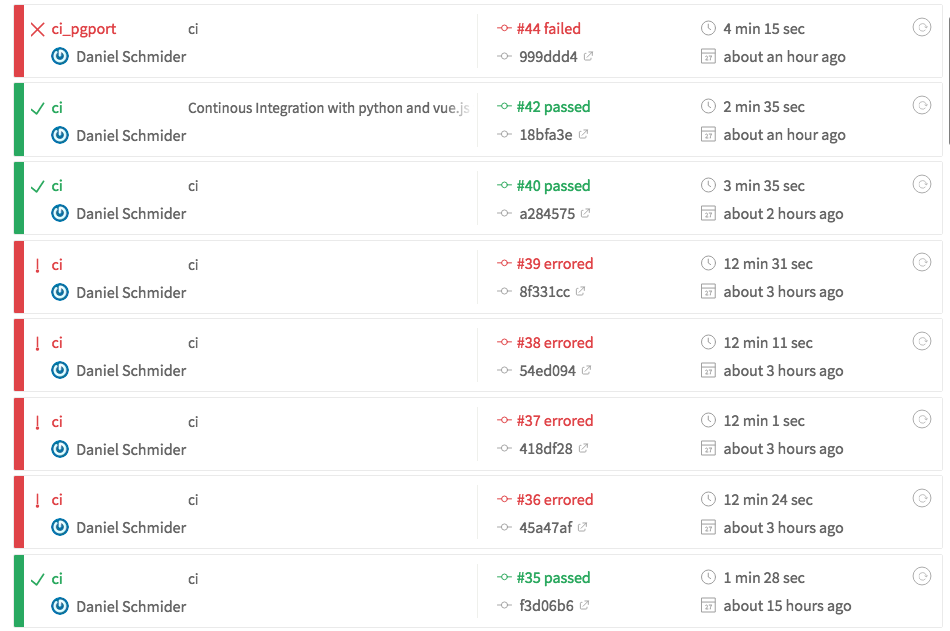
\includegraphics[width=1\textwidth]{travisv}
    \caption{TravisCI Version History}
    \label{fig:t1}
\end{figure}

\begin{figure}[H]
    \centering
    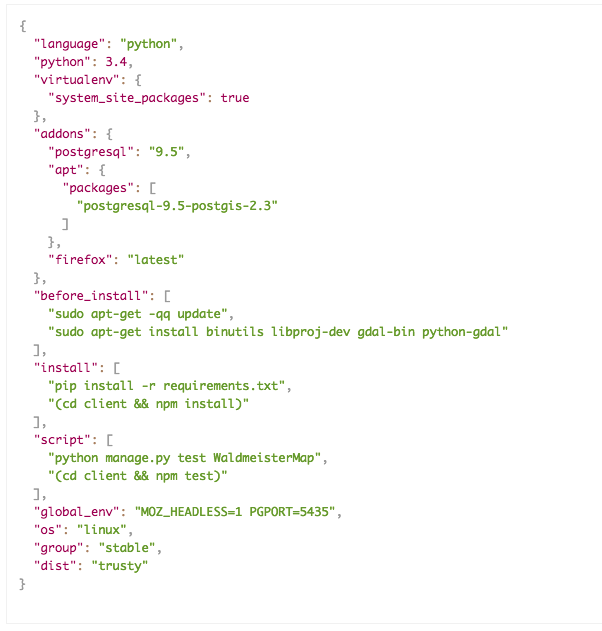
\includegraphics[width=1\textwidth]{travisc}
    \caption{Travis config .yaml, Version #45}
    \label{fig:t2}
\end{figure}

\begin{figure}[H]
    \centering
    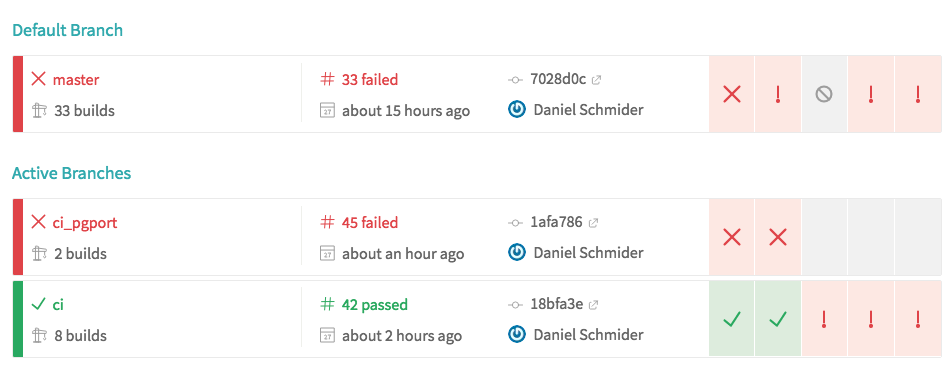
\includegraphics[width=1\textwidth]{travisb}
    \caption{Travis branches}
    \label{fig:t3}
\end{figure}

\section{Manuelle Tests}
\subsection{User-Szenario}
Das User-Szenario ist ein m\"oglicher Interaktionsablauf eines Users, welcher die Webapp "Waldmeister-Outdoors" verwendet. Es ist in die verschiedenen Schritte eingeteilt, welcher der User durchf\"uhrt.

1. Aufrufen der URL $\newline$
2. Scrollen, Zoomen der Map auf einen beliebigen Bereich $\newline$
3. Aufruf der "About" Seite $\newline$
4. \"Offnen der Map-Legende in einem separaten Tab $\newline$
5. Registrierung eines neuen Users, Eingabe von Benutzernamen und Passwort $\newline$
6. Login mit dem neu erstellten Benutzers $\newline$
7. Erstellung einer neuen privaten Benutzerfl\"ache $\newline$
8. Updaten der gerade erstellten Benutzerfl\"ache $\newline$
9. Erstellen einer neuen \"offentlicher Benutzerfl\"ache $\newline$
10. Erstellen einer zweiten \"offnentlicher Benutzerfl\"ache $\newline$
11. L\"oschen einer erstellten Benutzerfl\"ache $\newline$
12. Ausloggen des Benutzers $\newline$
13. Registrierung eines zweiten Benutzers $\newline$
14. Einloggen des zweiten Benutzers $\newline$
15. L\"oschungsversuch einer \"offentlichen Benutzerfl\"ache, welche vom ersten Nutzer erstellt wurde $\newline$
16. Erstellen einer \"offentlichen Benutzerfl\"ache $\newline$
17. Updaten der erstellen Benutzerfl\"ache, wechseln des Labels und \"offentlich auf privat $\newline$

\subsection{Testf\"alle}
Testfall A: $\newline$
Aufruf der URL $\newline$
Erwartet: Laden der Webapp$\newline$
Erf\"ullt: Ja/Nein$\newline$
$\newline$
Testfall B:$\newline$
Scrollen und Zoomen der Map$\newline$
Erwartet: Map scrollt durch drag & drop, zoomen durch Mousewheel oder Zoom Buttons
Erf\"ullt: Ja/Nein


\subsection{Ziel}

\subsection{Reproduktion}

\section{Resultate und Weiterentwicklung}
\subsection{Resultate}
User k\"onnen mittels der Webapp Waldmeister-Outdoors die Vegetationskundliche Karte erforschen und diese mit Ihrem momentanen Standort abgleichen. User k\"onnen, nachdem sie sich registriert haben, private und \"offentliche Benutzerfl\"achen erfassen und sie auf einem zentralen Server hinterlegen. Dies k\"onnen sowohl bisher nicht erfasste Waldstandorte, oder pers\"onliche Orte und Fl\"achen beschreiben, welche f\"ur Sie im Arbeitsalltag relevant sind. Solche Benutzerfl\"achen k\"onnen sie zwischen verschiedenen Ger\"aten (Im Feld und im B\"uro) abrufen oder mit anderen Personen teilen, sobald sie die Fl\"ache \"offentlich und daher von allen Usern abrufbar machen. $\newline$
Ebenfalls wurde erreicht die Geolocation auf der Karte darzustellen. Dies ist im Arbeitsalltag eine grosse Hilfe, und dient zur schnellen Orientierung und Auffindung von bestimmten eingetragenen Fl\"achen und Orten im Feld. $\newline$
Die Webapp kann sowohl auf Desktop Browsern wie von mobilen Ger\"aten verwendet werden und verh\"alt sich dank Vue.js responsive auf eine \"Anderung des Viewports, zum Beispiel wenn der Screen eines mobilen Ger\"ats w\"ahrend der Verwendung gedreht wird. $\newline$
Der Vegetationslayer und Benutzerfl\"achen-Layer und deren Label k\"onnen ein - und ausgeblendet werden, was zur \"Ubersicht beitragen kann. $\newline$
Alle Benutzeraccounts und deren Fl\"achen sind im Django Backend ersichtlich und k\"onnen als Superuser ver\"andert oder gel\"oscht werden. Wird ein Benutzer aus der Datenbank gel\"oscht, werden alle von ihm erstellten Benutzerfl\"achen ebenfalls automatisch gel\"oscht. Alle Passw\"orter von Benutzeraccounts werden gehasht in der Datenbank gespeichert. $\newline$
\subsection{M\"oglichkeiten der Weiterentwicklung}
\subsection{Vorgehen}

\section{Projektmanagement}
\subsection{Allgemeines}

\subsection{Prozessmodell}
Scrum wurde eingesetzt um bei der Entwicklung des Projekts agil vorzugehen. Transparenz, \"Uberpr\"ufung, Anpassung
Vereinfachte Form von Scrum
Sprints: Meetings (2-W\"ochentlich, W\"ochentlich, Intervalle)

Grund: Auf Issues reagieren sobald sie auftauchen und sie einfliessen lassen
In Scrum werden die Anforderungen in Form von Eigenschaften aus der Anwendersicht formuliert.
W\"ahrend eines Sprints sind keine \"Anderungen erlaubt, die das Sprintziel beeinflussen.
Product Backlog (github)

Sprint-Reviews (Emails, Drei Punkte)

Docker-Deployment bei Sprintende (als Testsystem ?)


\subsubsection{GitHub}

\subsection{Meilensteinplanung}
Meilensteine beschreiben Wichtige geplante Daten im Projektablauf. Im Projekt "Waldmeister-Outdoors" gibt es folgende Meilensteine:

1. Projektplan erstellen 18.4. $\newline$
2. Refactoring der Codebase, 2.5.$\newline$
3. Feature Freeze / Feature Demo 23.5. $\newline$
4. Abgabe Projekt 8.6. $\newline$

Bild, Gantt PDF

\subsection{Releases}
Als Release wird das Deployment der Webapp auf den Produktions Server bezeichnet. Grunds\"atzlich wird die Webapp auf einem Lokalen Testserver entwickelt und getestet. Bei einem Release wird die Lauff\"ahige Webapp auf das Livesystem portiert und \"offentlichen Usern zug\"anglich gemacht.
\subsection{Issues}
W\"ahrend dem Projekt und insbesondere w\"ahrend der Projektplanungsphase werden Issues erfasst, welche geplante Schritte, Funktionen oder Arbeitsschritte beschreiben.
\subsection{Prototypen}



\subsection{Aufwandsch\"atzung}
An Stakeholder
\subsubsection{Zeitplan}
Anzahl Tage in der Woche, Anzahl Wochen, Gesamtaufwand
An Stakeholder (\"ahnlich Meilensteinplanung)

\subsection{Risiken}
Technologien
Frameworks$\newline$
Mobile Limits $\newline$
Anzahl Objekte auf der Map, Performanceeinbussen $\newline$
Gps-Empfang und Internetempfang

\section{Projektmonitoring}
\subsection{Soll-Ist-Zeitvergleich}
\subsection{Code Statistics}

\section{Softwaredokumentation}
\subsection{Installation}
Um die App zu verwenden, sollte die Anleitung auf GitHub (Readme) verwendet werden, oder die .yml config Datei, um das Projekt auf einer Linux Machine zu builden. $\newline$
$\newline$
Github Repo klonen $\newline$ $\newline$
"npm install" $\newline$ $\newline$
"pip install -r requirements.txt" $\newline$ $\newline$
"npm start" im client folder startet den Vue-Server $\newline$ $\newline$
"python manage.py runserver" (als separates Window oder Tab) im root Folder startet den Django Server $\newline$ $\newline$
Damit Django die PostgreSQL Datenbank verwenden kann, m\"ussen die Werte in der settings.py angepasst werden, oder eine Datenbank mit dem Namen dschwaldmeister, user Postgres und Port 5432 erstellt werden. Von PostgreSQL soll auch die Extension postgis erzeugt werden. $\newline$
Mit "manage.py migrate" kann die Datenbank auf den neusten Stand gebracht werden, damit sie verwendet werden kann. $\newline$
Die App kann im Browser unter der angezeigten Adresse des Vue-Servers aufgerufen werden. $\newline$

Alternativ kann das Projekt mit dem Befehl "docker-compose build" in Dockercontainern gebuildet und mit "docker-compose up" ausgef\"uhrt werden. $\newline$
Das Projekt ist im Internet unter https://waldmeistermap.sifs0003.infs.ch/#/ deployt.

\subsection{Tutorial, Handbuch}
Registrierung: $\newline$
Um einen neuen Benutzer zu registrieren, muss ein bereits eingeloggter user sich ausloggen. Danach kann mit der Schaltfl\"ache "Register" ein neuer Account erstellt werden. Username und Passwort werden ben\"otigt, Email ist optional und kann leer gelassen werden.
$\newline$
Fl\"ache Erstellen:$\newline$
Ein eingeloggter User hat die M\"oglichkeit eine Neue Benutzerfl\"ache zu erstellen. Um dies zu tun, muss er auf die Schaltfl\"ache "Add" auf der linken Seite, unterhalb der Zoom Buttons klicken. Im Editiermodus kann er durch Klicks auf die Map neue Eckpunkte zu einem Polygon hinzuf\"ugen. Er kann die Fl\"ache schliessen, in dem er auf den ersten erstellten Eckpunkt klickt. Es \"offnet sich eine Dialogbox, in welchem der User der erstellten Fl\"ache einen Namen geben kann, welcher auf der Map erscheint. In dieser Dialogbox kann der User auch entscheiden, ob die Fl\"ache \"offentlich (f\"ur alle sichtbar) oder privat dargestellt werden soll (nur f\"ur den User sichtbar, welcher die Fl\"ache erstellt hat).

Fl\"ache Bearbeiten:$\newline$
Um eine bereits erstellte Fl\"ache zu bearbeiten und zu ver\"andern muss die zu \"andernde Fl\"ache angew\"ahlt werden, w\"ahrend der User, welcher die Fl\"ache erstellt hat, eingeloggt ist. Nur der User, der die Benutzerfl\"ache erstellt hat, kann diese Ver\"andern oder Updaten. Im Bearbeitungsmodus kann der User die Eckpunkte des Polygons beliebig verschieben. Durch einen Klick auf die Schaltfl\"ache "Upd" (Update), \"offnet sich die Dialogbox, um der Benutzerfl\"ache einen neuen Namen zu geben, oder Ihren Zustand von \"offentlich oder privat zu wechseln.

\subsection{Referenzhandbuch}
Vegetationslayer: Erster Layer oberhalb der Hintergrundkarte, welcher auf der Map dargestellt wird. Enth\"alt eingef\"arbte Polygone mit Labels welche einen Waldstandortstyp beschreiben. Die Daten, welche auf dem Vegetationslayer dargestellt werden, basieren auf der "Vegetationskundliche Kartierung der W\"alder im Kanton Z\"urich", bzw. der "Waldvegetationskarte".






